\documentclass[10pt, fullpage, a4paper, titlepage]{article}
\usepackage{graphicx, latexsym}
\usepackage{subfigure}
\usepackage{setspace}
\usepackage{amssymb, amsmath, amsthm}
\usepackage{bm}
\usepackage{epstopdf}
\usepackage{rotating} %used for \sidewaystable
\usepackage{apacite}
\usepackage{booktabs} %used for \toprule
\usepackage{multirow} 
\usepackage[]{hyperref}
\hypersetup{
    pdftitle={title of the pdf},
    pdfauthor={your name},
    pdfsubject={cool stuff},
    pdfkeywords={koala, chuck norris},
    bookmarksnumbered=true,     
    bookmarksopen=true,         
    bookmarksopenlevel=1,       
    colorlinks=true,            
    pdfstartview=Fit,           
    pdfpagemode=UseOutlines,      
    pdfpagelayout=TwoPageRight
}

\singlespacing
%\onehalfspacing
%\doublespacing



\title{Week 1\\ \small Exercise 1}
\author{Marta Sech}
\date{\today}
%\date{}

\begin{document}
\maketitle
\newpage

\section{An equation}
\begin{equation}
p(\pi) = \prod_{i=1}^{n-1}  \frac{\exp(\theta_{i})}{\sum_{l=i}^{n} \exp(\theta_{l})} 
\end{equation}
\newpage
\section{Some figures}
\begin{figure}[h]
	\begin{center}
		\resizebox{\textwidth}{!}{
		\subfigure[Histogram]{
		\label{histogram:a}
	  			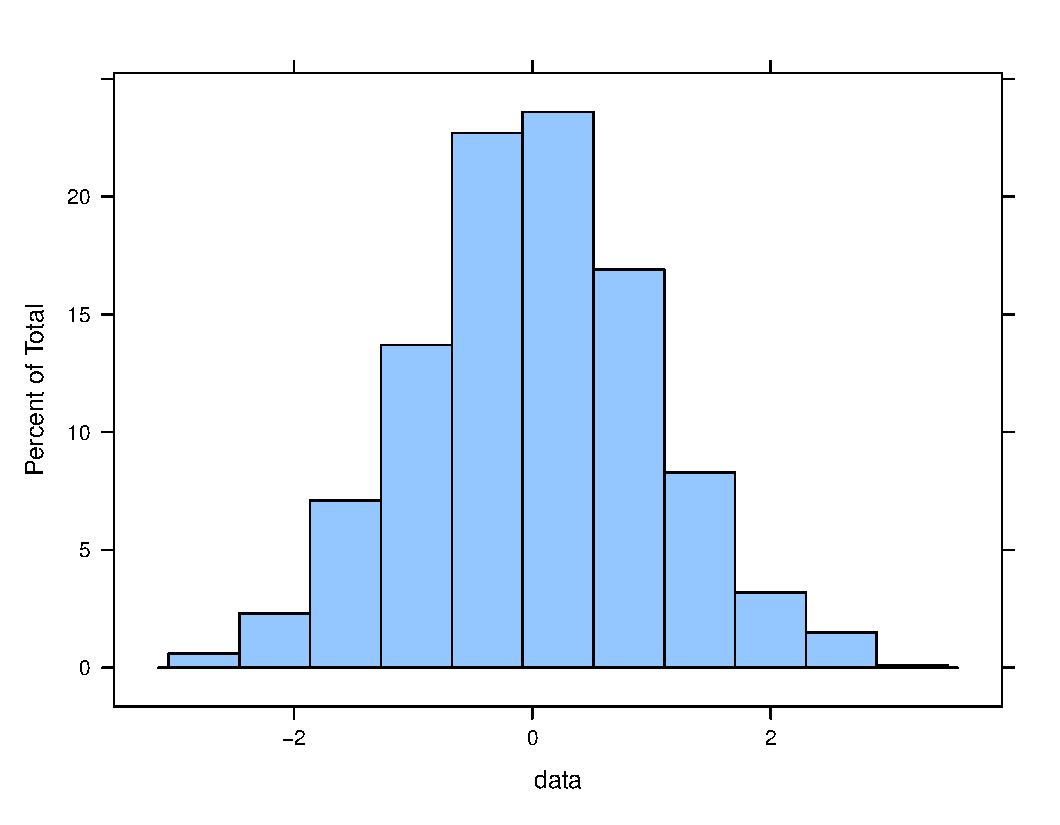
\includegraphics[scale=.5]{histogram.pdf}
	                 }
			\subfigure[Densityplot]{
 		        \label{densityplot:b}
				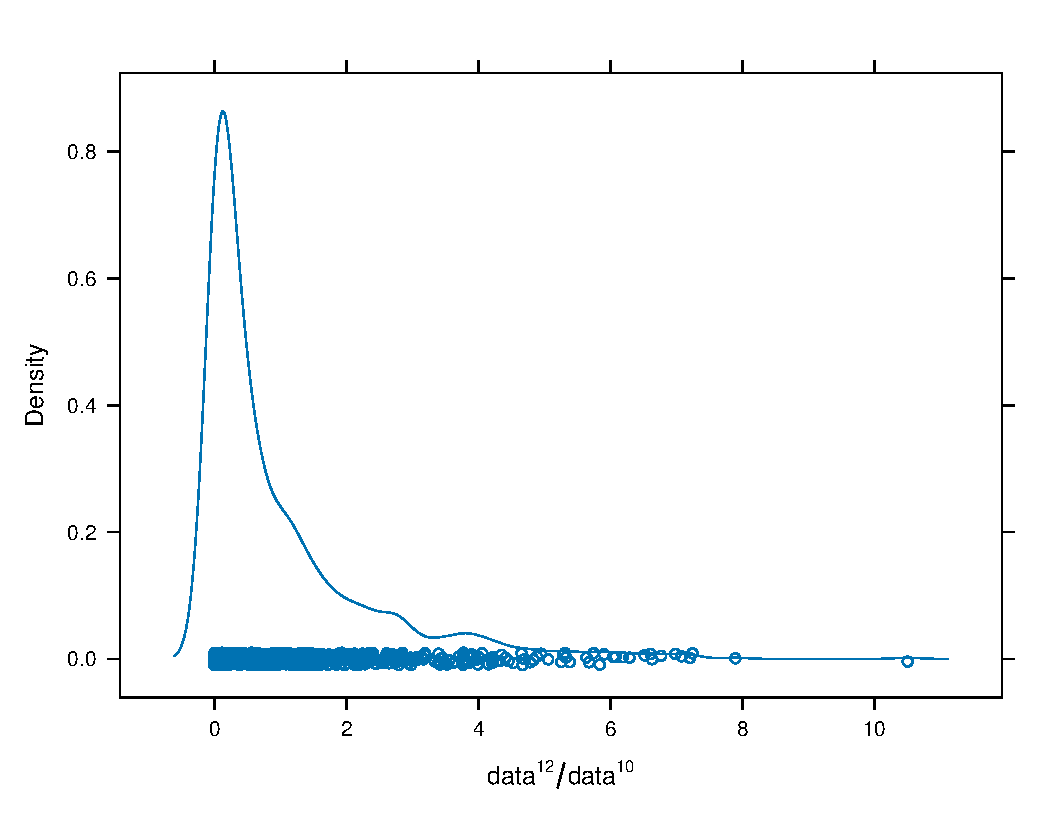
\includegraphics[scale=.5]{densityplot.pdf}
		        }
		} \\ 	
				\resizebox{\textwidth}{!}{
			 \subfigure[Stripplot]{
  		        \label{stripplot:c}
	 			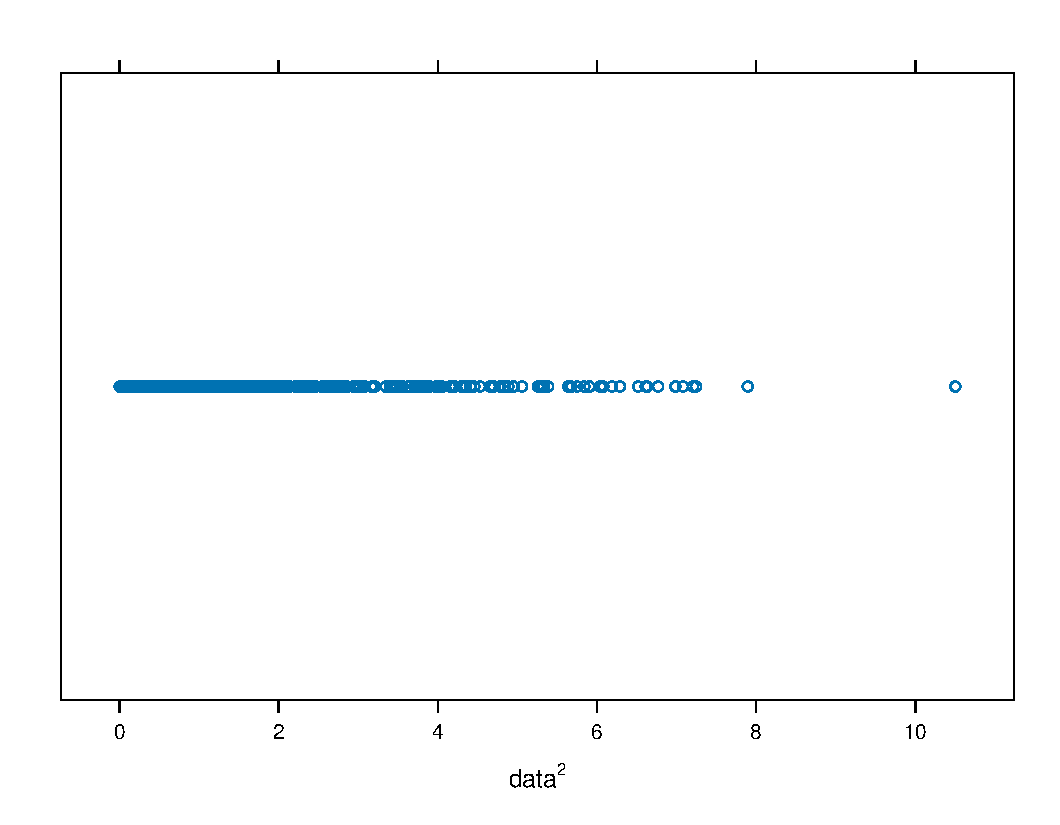
\includegraphics[scale=.5]{stripplot.pdf}
			 }
			 \subfigure[Boxplot]{
 		        \label{boxplot:d}
				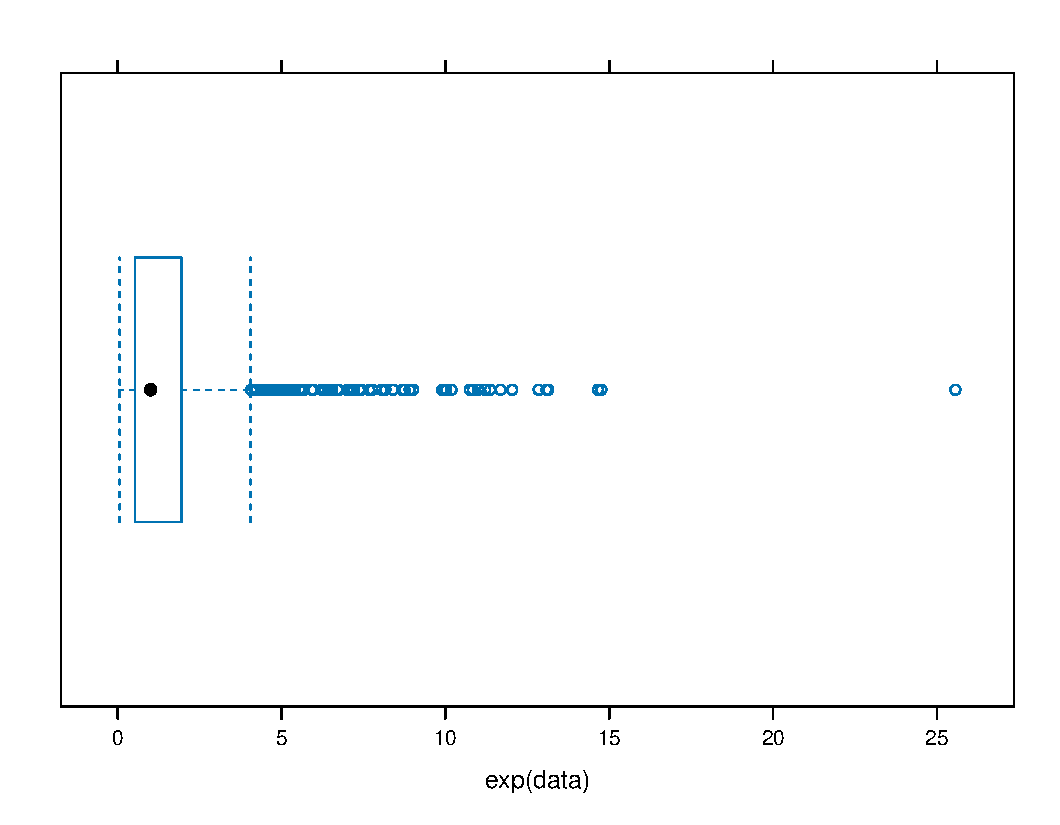
\includegraphics[scale=.5]{boxplot.pdf}}
			 }
		}
	\end{center}
	\caption{Different plots of the same data, sometimes transformed. No particular objective other than it being an exercise.}
	\label{Fig1}
\end{figure}
\newpage
\section{A table}
\begin{table}[h!]
	\centering
	\caption{The same data, but now in a table. Only the first six rows are displayed.}
	\begin{tabular}{rrrrr}
  		\hline
		 & data & squared1 & squared2 & exponent \\ 
		\hline
		1 & -0.56047565 & 0.314132950 & 0.314132950 & 0.5709374 \\ 
  		2 & -0.23017749 & 0.052981677 & 0.052981677 & 0.7943926 \\
		3 & 1.55870831  & 2.429571609 & 2.429571609 & 4.7526783 \\
  		4 & 0.07050839  & 0.004971433 & 0.004971433 & 1.0730536 \\
  		5 & 0.12928774  & 0.016715318 & 0.016715318 & 1.1380175 \\
  		6 & 1.71506499  & 0.941447909 & 2.941447909 & 5.5570366 \\
		\hline
	\end{tabular}
\end{table}

\newpage
\section{AI generated fairytale}
The Enchanted Garden and the Luminous Dove

Once, in a land covered by mists and whispers, there lay an enchanting garden hidden behind a great stone wall. No one knew who had built the wall or why, but one thing was for certain – nobody had ever seen what was behind it.

A little girl named Clara lived in a village nearby. Fueled by curiosity and tales of magical creatures, she often dreamt of the wonders that the walled garden might hold. One day, unable to resist its lure any longer, she decided to find a way in.

As she approached the towering stone barrier, she noticed a tiny gap just big enough for her to peek through. The garden inside was bathed in a shimmering golden light, unlike any she had ever seen. To her amazement, in the center stood a magnificent tree with leaves that glittered as if they were made of starlight. And resting on one of its branches was a dove, glowing with the same luminous hue.

Before she could process this beautiful sight, the dove spoke to her in a voice as soft as the wind, "To enter the garden, one must share a pure and selfless desire."

Clara, with her heart pounding, whispered her wish, "I wish for everyone in my village to be happy and free from suffering."

The massive stone door, seemingly of its own accord, began to open. The luminous dove flew to Clara and rested on her shoulder. "Your wish is genuine, and so you may enter," it said.

Inside, the garden was more wondrous than Clara had ever imagined. Flowers sang in soft harmonies, and a gentle breeze carried the sweetest of fragrances. Every step she took made the grass shimmer with colors she'd never seen before.

The dove explained that this was an Enchanted Garden, a place where one’s purest wishes could come true. But, there was a catch. To make her wish a reality, Clara had to plant a seed from the magical tree in her village and care for it with unwavering love and dedication.

Clara accepted the challenge. With the seed safely tucked in her pocket and the dove guiding her, she returned to her village.

Years went by, and with Clara's love, the seed grew into a magnificent tree, similar to the one in the Enchanted Garden. With its growth, joy and happiness blossomed in the village like never before.

Clara's selfless wish not only transformed her village but also changed her. She became known as the Keeper of Joy, teaching future generations about love, compassion, and the magic of selfless wishes.

And so, in a village once shadowed by mystery, there stood a tree that bore witness to the pure heart of a girl and her luminous companion, reminding everyone that magic was always just a wish away.

\subsection{A subsection}
Text to be inserted in the subsection



\end{document}